\documentclass[11pt, a4paper]{article}

\usepackage{amsmath}
\usepackage{amsfonts} %Matheschriften
\usepackage{amssymb} %Mathesymbole
%\usepackage{mathptmx} % Einstellung für Schriften und Sonderzeichen in mathematischen Umgebungen
                        % ändert SChriftfont
\usepackage{wasysym} % Stellt diverse Sonderzeichen bereit
\usepackage{siunitx}
\usepackage{float}
\usepackage{microtype}
\usepackage{graphicx}
\usepackage{hyperref}
\usepackage{xcolor}
\usepackage[section]{placeins}
% allows for temporary adjustment of side margins
\usepackage{changepage}
\usepackage{rotating}


\usepackage[ngerman]{babel}
\addto\captionsngerman{%
 \renewcommand{\abstractname}{Einleitung}}

\title{Versuch 2: Interferometer}
\author{Team 4-11: Jascha Fricker, Benedict Brouwer}

\begin{document}
    \maketitle

    \tableofcontents

    \newpage

    \section{Einleitung}

    Interferometer werden im der Messtechnik für viele verschiedene Aufgaben benutzt. Das Micherlson-Interferometer ist eines der bekanntesten Arten von Interferometer, welches unter anderem beim Michelson-Morley Experiment zum Bestimmung der Äther-Geschwindigkeit benutzt wurde. In diesem Versuch benutzen wir es um den Brechungsindex von Plexiglas und Luft zu bestimmen.

    \section{Experimenteller Aufbau}

    Das Michelson Interferometer, wie in der Abbildung \ref{fig:auf} gezeigt, besteht aus einem Laser, der durch einen halbdurchsichtigen Spiegel als Strahlteiler in zwei unterschiedliche Wege aufgespalten wird. Am Ende jedes Armes steht ein Spiegel, der das Laserlicht wieder zurück zum Strahlteiler reflektiert. In unserem Versuchsaufbau war einer dieser Spiegel durch eine Schraube verschiebbar. Beide zurückgeworfenen Strahlen interferieren zu einem von den optischen Weglängen der zwei Arme abhängigem Interferenzmuster.

    \begin{figure}
        \centering
        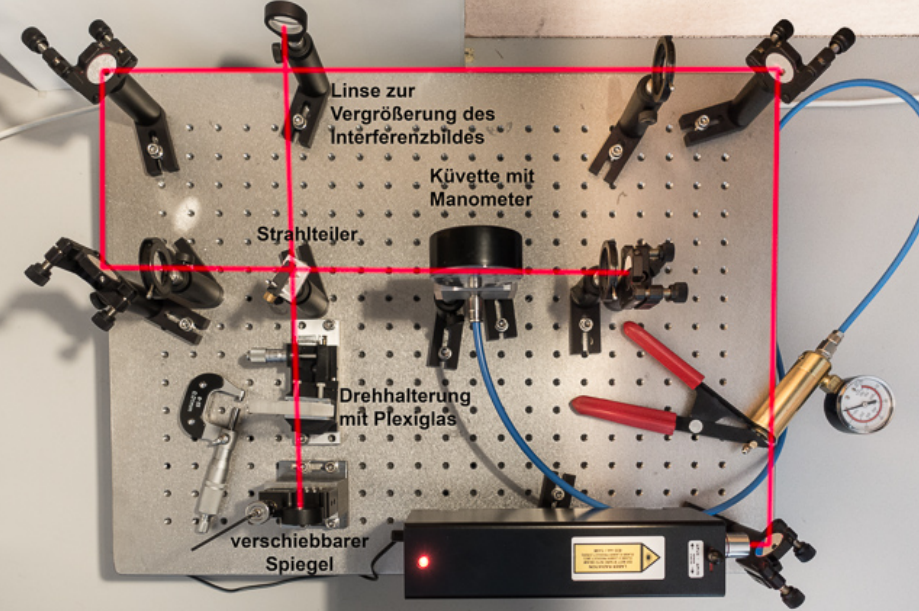
\includegraphics[width=0.8\textwidth]{Screenshot 2023-03-13 5.35.50 PM.png}
        \caption{Experimenteller Aufbau aus der Aufgabenstellung \cite{intauf}}
        \label{fig:auf}
    \end{figure}

    \section{Theorie}
    \subsection{Ganghöhenbestimmung} \label{sec:gang}

    Mithilfe der Formeln
    \begin{align}
        \Delta s = \frac{N \cdot \lambda}{2}
    \end{align}
    kann man die Verschiebung des Spiegels $\Delta s$ durch die Anzahl der Maxima $N$ und berechnen. Für die Ganghöhe der Schraube wollen wir den Abstand pro Umdrehung
    \begin{align}
        g = \frac{\Delta s}{\Delta x} = \frac{N \lambda}{2 \Delta x} = \frac{2500 \lambda}{2 S} \label{eq:gang}
    \end{align}
    haben, wobei $x$ Anzahl der Umdrehungen und $S = \frac{x}{50}$ die Anzahl an Strichen für 50 Interferenzmaxima ist. 

    \subsection{Brechungsindex Luft}
    Mit folgenden Formeln sind Brechungindex $n$, Druck $p$ und Anzahl gezählter Maxima $N$ verknüpft
    \begin{align}
        N \cdot \lambda &= 2 l \cdot \Delta n \label{eq:n}\\
        n &= 1 + \frac{\chi}{T} p \label{eq:luft} \\ 
        N \cdot \lambda &= 2 l \cdot \frac{\chi}{T} \Delta p
    \end{align}
    wobei $l$ die Länge der evakuierbaren Kammer ist.

    \subsection{Brechungsindex Plexiglas}
    Durch Drehung der Plexiglsscheibe mit Dicke $d$ um Winkel $\alpha$ kann der Brechungsindex $n$ bestimmt werden.
    \begin{align}
        N \cdot \lambda &= 2 \cdot h \cdot \left(1 - n - \cos(\alpha) + \sqrt{n^2 - \sin^2(\alpha)}\right)\label{fitplex} \\
        tan(\alpha) &= \frac{x + c}{d} \label{Winkelum}
    \end{align}
    wobei $N$ die Anzahl an Maxima $x$ die Länge der Schraube und $d$ der Abstand der Schraube vom Drehpunkt ist.

    \section{Experimentelles Vorgehen}

    \subsection{Ganghöhe}
    In diesem Experiment wurde die Ganghöhe der Schraube gezählt, mit der der Spiegel am ende einer der Arme der Interferrometer verschoben werden konnte. Dies wurde gemacht, indem drei mal die benötigte Umdrehung der Schraube gemessen wurde, um 100 Interferenzmaxima zu beobachten. Wir haben auch den Wert bei 50 Maxima aufgeschrieben. Aus diesen Werten lässt sich die Ganghöhe wie in \ref{sec:gang} beschrieben berechnen.

    \subsection{Brechungindex Luft}
    Bei diesem Versuch wurde in einen der Arme des Interferometer eine evakuierbare Kuvette platziert. Diese wurde bis zu einem relativen Druck von $-0.8 \si{\bar} $ lehrgepumpt und anschließend wurde bei jedem dritten Interferenzmaximum, welche durch das langsame Eindringen von Luft durch Undichtigkeiten im Aufbau entstanden, der aktuelle Luftdruck gemessen.

    \subsection{Brechungindex Plexiglas}
    Hier wurde in einen der Arme des Interferometer eine entlag der vertikalen Achse drehbare Plexiglasscheibe platziert. Diese wurde durch eine Mikrometerschraube langsam vom einen zu anderen Anschlag gedreht und dabei, je nach Position, jedes 10., 5., 3., oder 1., Maximum im Interfenzmuster der Wert der Mikrometerschraube aufgeschrieben.



    \section{Ergebnisse}
    \subsection{Ganghöhe}

    Aus den 3 Messreihen lässt sich mit der Gleichung \ref{eq:gang} eine Ganghöhe des Spiegels von
    \begin{align}
        g = 47.58(21) \si{\micro\metre}
    \end{align}
    pro Schraubendrehung bestimmen. So ist jeder Strich eine verschibung um etwa einen Mikrometer. Als Fehler wurden wegen der analogen Messung eine Ungenauigkeit von $0.21$ Einheiten in der Schraubenstellung angenommen. Die Abweichung zum Idealwert von $50 \si{\micro\meter}$ kann durch den Backlash bei der Drehung, ein verbiegen der Halterung durch einseitige Belastung bei Drehung mit dem Imbusschlüssel oder ein ungenaues Zählen erklärt werden.
    
   
    \subsection{Brechungsindex Luft}
    Mit der Gleichung \ref{eq:n} und einer Küvettenlänge von $l = 49,4(1) \si{\milli\metre}$ konnte aus der Anzahl der Maxima die relative Änderung des Brechungsex $\Delta n$ berechnet werden.
    Durch einen Fit der Formel \ref{eq:luft}, wie im Graphen \ref{fig:druck} gezeigt, kann die Proprtionalitätskonstante zwischen Brechungsindex und Luft $\chi$ und der Brechungsindex $n$
    \begin{align}
        \chi = 7,52(11) \cdot 10^{-7} \si{\kelvin\per\pascal} \\
        n = 1 + \frac{7,52(11) \cdot 10^{-7} \si{\kelvin\per\pascal}}{T} \cdot p
    \end{align}
    bestimmt werden. Berücksichtigt wurden Unsicherheiten beim Luftdruck, bei der Längenmessung der evakuierten Kammer und bei der Temperatur, die zu Zeit der Messung $22.7(1) ^{\circ}C$ betrug. Als Theoriewert (Siehe \cite{theoluft}) konnte der Brechungsindex von Luft $n = 1.00027653$ bei $15 ^{\circ}C$, $101325 \si{\pascal}$ und $450$ ppm C02 gefunden werden. Aus diesen Werten lässt sich $\chi = 7,864 \cdot 10^{-7}  \si{\kelvin\per\pascal}$ berechnen, welches nahe beim von uns berechneten Wert, aber nicht im Konfidenzintervall liegt.
    
    \begin{figure}
        \centering
        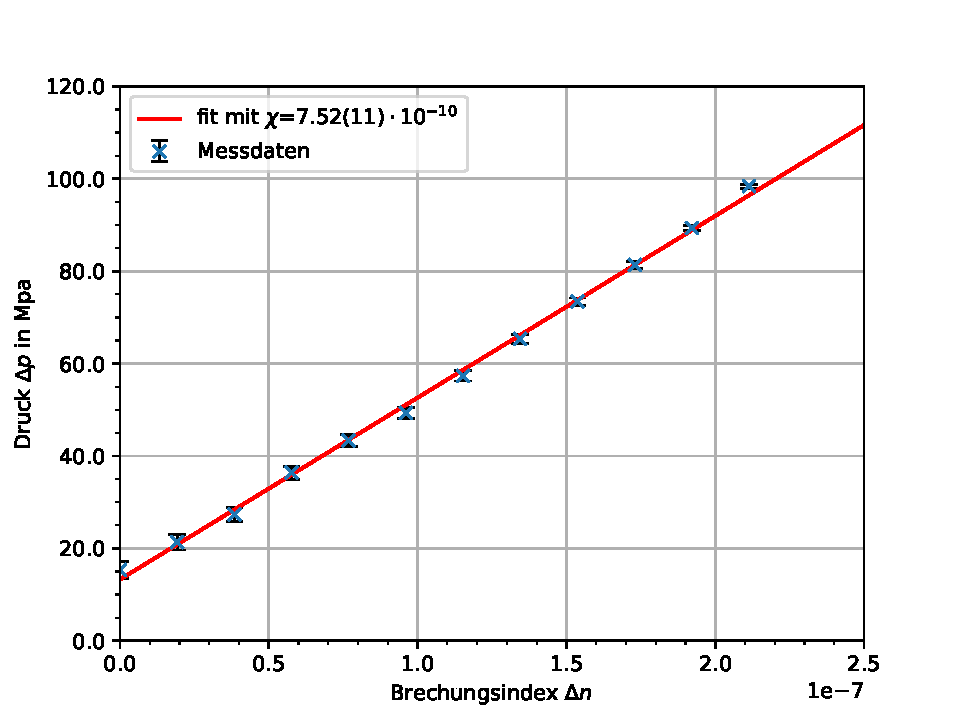
\includegraphics[width=0.8\textwidth]{./plots/druck.pdf}
        \caption{Druckabhänger Brechungindex}
        \label{fig:druck}
    \end{figure}

    \subsection{Brechungsindex der Plexiglasplatte}
    Um den Brechungsindex einer Plexiglasplatte zu bestimmen wird diese auf einem rotierenden Tisch, dessen Winkel zum Strahl mit einer Arretierungsschraube eingestellt werden kann, montiert.
    Aus den abgelesenen Werten kann mit \ref{Winkelum} und einer Helbelarmlänge von $d = 28$ mm Der Winkel zum Strahl berechnet werden.
    Die gemessenen Werte wurden nun in Graph \ref{fig:plexiplot} mit Funktion \ref{fitplex} gefittet. Dabei erhielten wir für den Brechungsindex einen Wert von
    \begin{align}
        n = 1,46337(95)
    \end{align}
    was vergleichbar mit dem Literaturwert von $n_{lit} = 1,5007$ \cite[Siehe:]{refdat} ist.
    \begin{figure}[!h]
        \centering
        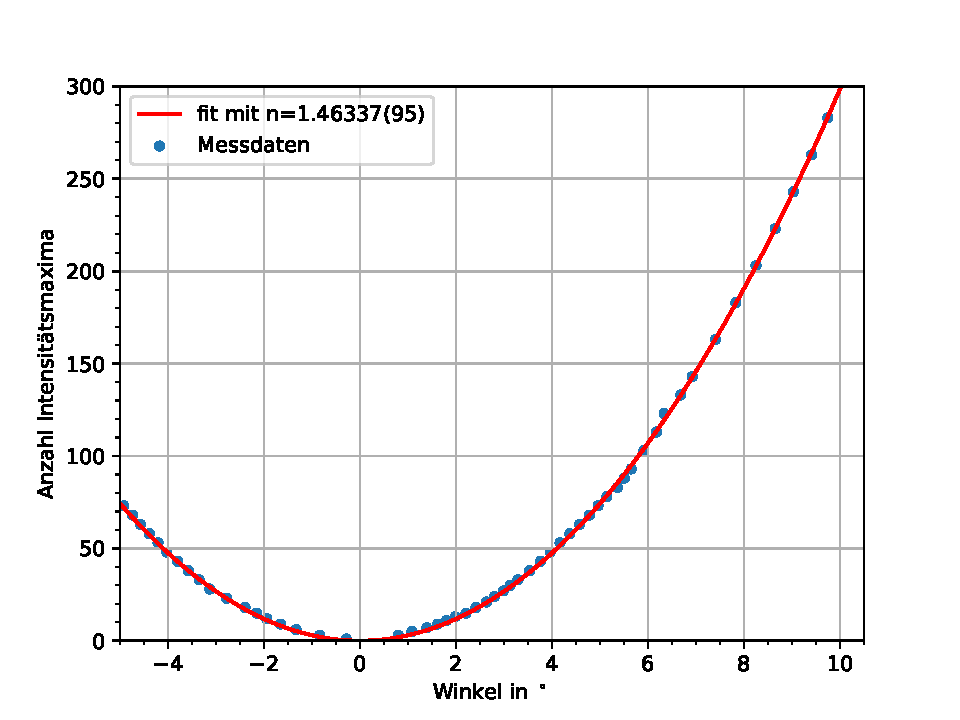
\includegraphics[width=\textwidth]{./plots/plexi.pdf}

        \caption{Durchlaufene Intensitätsmaxima in Bezug auf den Drehwinkel des Tisches}
        \label{fig:plexiplot}
    \end{figure}

    \section{Diskussion}
    Im Versuch mit dem Michelsen Interferometer konnte erfolgreich die Ganghöhe der Spiegelarretierungsschraube bestimmt werden.
    Auch der Brechungsindex der Luft konnte als Funktion angegeben werden und liegt in einem sinvollen Bereich.
    Bei der Bestimmung des Brechungsindex der Plexiglasscheibe wurde ein Wert bestimmt, der die richtige Größenordnung hat. Ob er genau stimmt, kann nicht überprüft werden, da das genaue Material nicht bekannt ist.
    \bibliographystyle{plain}
    \bibliography{literature}
    % https://refractiveindex.info/?shelf=other&book=pmma_resists&page=Microchem495

\end{document}